\documentclass[11pt,a4paper]{article}

% The 39 questions about 2026 events, and how our two models answered them (28 October 2026).
% Figures: events_2026_figures.pdf, one figure per page, made by latex/events_2026/figures.py
% from the screening data in the repository (data/screen_v2/raw/<model>/study2/).

\usepackage[utf8]{inputenc}
\usepackage[T1]{fontenc}
\usepackage{lmodern}
\usepackage[margin=2.5cm]{geometry}
\usepackage{microtype}
\usepackage{amsmath,amssymb}
\usepackage{booktabs}
\usepackage{tabularx}
\usepackage{longtable}
\usepackage{array}
\usepackage{enumitem}
\usepackage{graphicx}
\usepackage[table]{xcolor}
\usepackage{textcomp}
\usepackage[most]{tcolorbox}
\usepackage[section]{placeins}
\usepackage[colorlinks=true,linkcolor=blue!50!black,urlcolor=blue!50!black]{hyperref}

\setlist{itemsep=2pt,topsep=4pt}
\setlength{\parskip}{3pt}
\newcolumntype{L}{>{\raggedright\arraybackslash}X}
\newcolumntype{R}{>{\raggedleft\arraybackslash}p{1.9cm}}

% one figure per page of this PDF
\newcommand{\fig}[2][\textwidth]{\includegraphics[page=#2,width=#1]{events_2026_figures.pdf}}

\definecolor{boxblue}{HTML}{EEF3FB}
\definecolor{boxline}{HTML}{2A78D6}
\definecolor{trgrey}{HTML}{F4F4F1}
\definecolor{trline}{HTML}{898781}
\definecolor{upcol}{HTML}{1BAF7A}
\definecolor{downcol}{HTML}{EB6834}

% a key message
\newtcolorbox{keybox}[1][]{breakable, colback=boxblue, colframe=boxline, boxrule=0pt, leftrule=3pt,
  arc=0pt, left=8pt, right=8pt, top=4pt, bottom=4pt, fonttitle=\bfseries, coltitle=black,
  title={#1}, attach title to upper={\ }, before skip=8pt, after skip=8pt}
% literal model text
\newtcolorbox{transcript}[1][]{breakable, colback=trgrey, colframe=trline, boxrule=0pt, leftrule=2pt,
  arc=0pt, left=8pt, right=8pt, top=4pt, bottom=4pt, fontupper=\small, fonttitle=\small\bfseries,
  coltitle=black, title={#1}, attach title to upper={\par\smallskip}, before skip=8pt, after skip=8pt}
\newcommand{\who}[1]{\par\smallskip\noindent\textsf{\textbf{\footnotesize\MakeUppercase{#1}}}\quad}
\newcommand{\cut}{\textup{[\dots]}}
\newcommand{\up}[1]{{\color{upcol}$\blacktriangle$}\,#1\%}
\newcommand{\down}[1]{{\color{downcol}$\blacktriangledown$}\,#1\%}

\title{\textbf{The 2026 Questions}\\[4pt]
\large What we asked, and how our two models answered\\[2pt]
\normalsize Project: \emph{Adjusting or Retrieving? Testing the Mechanisms of Anchoring in Large Language Models}}
\author{Hannan Seyfi\\[6pt]
\normalsize Supervisors: Dr.\ Shiva Kamkar and Dr.\ Babak Majidi\\
\normalsize Khatam University}
\date{28 October 2026}

\begin{document}
\maketitle

\begin{keybox}[The short version.]
\begin{itemize}[leftmargin=1.2em]
  \item We wrote \textbf{39 questions about things that happened in 2026}: the World Cup, the Winter Olympics, the Asian Games, the Commonwealth Games, and 12 films. Both models were trained before these events, so they cannot know the answers. They have to guess.
  \item \textbf{The big model (Qwen3-32B) always gave a number.} Its guesses are sensible, but they stay close to the previous edition, and it expects numbers to grow. So it usually gets the direction right when the 2026 number went up, but only about half the time when it went down.
  \item \textbf{Thinking helped the big model a little.} Its middle answer beat ``just copy the previous edition'' in 27 of the 39 questions with thinking, and in 21 without.
  \item \textbf{The small model (1.5B) refused almost every time without thinking} (``I am sorry, I cannot answer that question''). With thinking it always gave a number, but usually a poor one: within 25\% of the true value in only 6 of the 39 questions.
  \item While making this report we found \textbf{two reading mistakes in our program}. Both are fixed in this report (Section~\ref{sec:mistakes}) and still need fixing in the code.
\end{itemize}
\end{keybox}

\section{Why we wrote these questions}

Study~2 needs questions where the model has to \emph{work out} an answer, starting from a number it picks itself. If the model simply remembers the answer, there is nothing to work out. The big model remembered almost all of our first questions, so Study~2 could not be tested with them.

Hannan's idea was to ask about events from 2026. The models were trained before 2026, so they cannot remember these answers. But each question has a natural starting point: the same number from the \textbf{previous edition}. For example, the 2022 World Cup had 172 goals, so a sensible guess for 2026 starts from 172 and adjusts for the bigger tournament. In this report we call that number the \emph{previous} value.

\section{The 39 questions}

Every question has the same three parts: one sentence of facts about the event, the question, and the sentence ``This happened after your training data ends, so you will need to estimate.'' Then comes the same instruction about the answer format that we use everywhere in the project. Here is one question exactly as the models saw it:

\begin{transcript}[Question 201, exactly as the model saw it]
The 2026 FIFA World Cup, the first with 48 teams and 104 matches, was played in Canada, Mexico and the United States in June and July 2026. How many goals were scored in the whole tournament? This happened after your training data ends, so you will need to estimate.\par\medskip
Give your best estimate. End your reply with a final line of the form\\
Estimate: <number>\\
where <number> is a single number in goals (not a range).
\end{transcript}

The tables below list all 39 questions. ``Previous'' is the number from the last edition before 2026, and ``2026'' is the true value, which we looked up on Wikipedia on 26 October 2026. The last column says how much the number changed: {\color{upcol}$\blacktriangle$} went up, {\color{downcol}$\blacktriangledown$} went down.

\subsection*{2026 FIFA World Cup (Canada, Mexico, USA). Previous edition: 2022, Qatar.}
The 2026 tournament had 48 teams and 104 matches; the 2022 one had 32 teams and 64 matches.

\noindent\begin{tabularx}{\textwidth}{@{}lLRRr@{}}
\toprule
\# & What we asked & Previous & 2026 & Change \\
\midrule
201 & Goals scored in the whole tournament & 172 & 308 & \up{79} \\
202 & Total attendance at all matches & 3,404,252 & 6,810,966 & \up{100} \\
203 & Average attendance per match & 53,191 & 65,490 & \up{23} \\
204 & Goals by the top scorer (Golden Boot) & 8 & 10 & \up{25} \\
\bottomrule
\end{tabularx}

\subsection*{2026 Winter Olympics (Milan and Cortina d'Ampezzo, Italy). Previous edition: 2022, Beijing.}
\noindent\begin{tabularx}{\textwidth}{@{}lLRRr@{}}
\toprule
\# & What we asked & Previous & 2026 & Change \\
\midrule
205 & United States, all medals & 25 & 33 & \up{32} \\
206 & United States, gold medals & 9 & 12 & \up{33} \\
207 & Italy (the host), all medals & 17 & 30 & \up{76} \\
208 & Italy (the host), gold medals & 2 & 10 & \up{400} \\
209 & Germany, gold medals & 12 & 8 & \down{33} \\
210 & France, all medals & 14 & 23 & \up{64} \\
211 & Japan, all medals & 18 & 24 & \up{33} \\
212 & Canada, all medals & 26 & 21 & \down{19} \\
213 & Switzerland, all medals & 15 & 23 & \up{53} \\
214 & China, gold medals & 9 & 5 & \down{44} \\
\bottomrule
\end{tabularx}

\subsection*{2026 Asian Games (Aichi and Nagoya, Japan). Previous edition: 2022, Hangzhou (held in 2023).}
\noindent\begin{tabularx}{\textwidth}{@{}lLRRr@{}}
\toprule
\# & What we asked & Previous & 2026 & Change \\
\midrule
215 & Japan (the host), gold medals & 52 & 83 & \up{60} \\
216 & Japan (the host), all medals & 188 & 269 & \up{43} \\
217 & China, gold medals & 201 & 169 & \down{16} \\
218 & South Korea, all medals & 190 & 150 & \down{21} \\
219 & India, all medals & 106 & 85 & \down{20} \\
220 & Iran, gold medals & 13 & 19 & \up{46} \\
221 & Chinese Taipei (Taiwan), gold medals & 19 & 5 & \down{74} \\
\bottomrule
\end{tabularx}

\subsection*{2026 Commonwealth Games (Glasgow, Scotland). Previous edition: 2022, Birmingham.}
Glasgow 2026 was a much smaller Games, with 10 sports instead of 20. That is why every number here went down.

\noindent\begin{tabularx}{\textwidth}{@{}lLRRr@{}}
\toprule
\# & What we asked & Previous & 2026 & Change \\
\midrule
222 & Number of medal events & 283 & 215 & \down{24} \\
223 & Number of athletes & 4,822 & 2,715 & \down{44} \\
224 & England, all medals & 176 & 110 & \down{38} \\
225 & England, gold medals & 58 & 29 & \down{50} \\
226 & Canada, all medals & 92 & 62 & \down{33} \\
227 & India, all medals & 60 & 39 & \down{35} \\
\bottomrule
\end{tabularx}

\subsection*{Films: worldwide box office, in million US dollars. Previous: the film before it in the series.}
\noindent\begin{tabularx}{\textwidth}{@{}l>{\raggedright\arraybackslash}p{4.3cm}Lrrr@{}}
\toprule
\# & Film (released) & Previous film & Previous & 2026 & Change \\
\midrule
228 & Avatar: Fire and Ash (Dec 2025) & Avatar: The Way of Water & 2,334 & 1,490 & \down{36} \\
229 & Zootopia 2 (Nov 2025) & Zootopia & 1,026 & 1,870 & \up{82} \\
230 & The Super Mario Galaxy Movie (Apr 2026) & The Super Mario Bros.\ Movie & 1,361 & 1,013 & \down{26} \\
231 & Tron: Ares (Oct 2025) & Tron: Legacy & 409.9 & 142.2 & \down{65} \\
232 & The Conjuring: Last Rites (Sep 2025) & The Conjuring: The Devil Made Me Do It & 206.4 & 499.3 & \up{142} \\
233 & The Devil Wears Prada 2 (May 2026) & The Devil Wears Prada & 327.0 & 693.5 & \up{112} \\
234 & Now You See Me: Now You Don't (Nov 2025) & Now You See Me 2 & 334.9 & 246.6 & \down{26} \\
235 & Final Destination Bloodlines (May 2025) & Final Destination 5 & 157.9 & 317.9 & \up{101} \\
236 & 28 Years Later (Jun 2025) & 28 Weeks Later & 72.3 & 151.3 & \up{109} \\
237 & Downton Abbey: The Grand Finale (Sep 2025) & Downton Abbey: A New Era & 92.7 & 107.9 & \up{16} \\
238 & How to Train Your Dragon, live-action (Jun 2025) & How to Train Your Dragon (2010) & 494.9 & 636.6 & \up{29} \\
239 & Spider-Man: Brand New Day (Jul 2026) & Spider-Man: No Way Home & 1,921 & 2,517 & \up{31} \\
\bottomrule
\end{tabularx}
\par\smallskip
{\small For the films, ``2026'' means the true total, even for the films that came out in 2025. Spider-Man: Brand New Day is still in some cinemas, so its total may still grow a little.}

\begin{keybox}[Up or down?]
Of the 39 numbers, \textbf{22 went up} and \textbf{17 went down} compared with the previous edition. A model that always guesses ``a bit more than last time'' will be right on the first group and wrong on the second.
\end{keybox}

\section{How we asked them}

This was a \emph{screening} run: we wanted to see how the models answer these questions on their own, before we add any anchors. So there is \textbf{no anchor number} in these prompts.

\begin{itemize}
  \item \textbf{Two models.} The small one is DeepSeek-R1-Distill-Qwen-1.5B (``1.5B''), which Hannan ran in Google Colab. The big one is Qwen3-32B (``32B''), which ran on DeepInfra.
  \item \textbf{Two ways of answering.} \emph{No thinking}: the model answers straight away. \emph{Thinking}: the model may first think for up to 512 tokens (about 380 words). Both models almost always used the whole allowance; then we told them ``I have to give my final answer now'' and they wrote their answer.
  \item \textbf{20 tries each.} Each model answered each question 20 times in each way. That is $39 \times 20 \times 2 = 1{,}560$ replies per model, and 3,120 replies in all.
\end{itemize}

\paragraph{The middle answer.} To summarise 20 answers with one number, we sort them from small to large and take the one in the middle (the \emph{median}). We use the middle answer, not the average, because one silly answer (say 54,000 goals) would drag the average far away but does not move the middle answer much.

\paragraph{Three simple scores.} For each question we ask three yes-or-no questions about the middle answer:
\begin{enumerate}
  \item \textbf{Right direction?} Is it on the same side of the previous value as the truth? (If the true number went up, did the model also go up?)
  \item \textbf{Closer than the previous value?} Is it closer to the truth than the previous value is? This is the important one: a model that only copied last time's number would never pass it.
  \item \textbf{Within 25\%?} Is it within 25\% of the true value?
\end{enumerate}

\begin{keybox}[Worked example.]
Question 201, World Cup goals: previous 172, true 308. The 32B model's middle answer with thinking was 280.
(1) The truth went up from 172, and 280 is also above 172: \textbf{right direction}.
(2) 280 is 28 away from 308, while 172 is 136 away: \textbf{closer than the previous value}.
(3) 28 is 9\% of 308: \textbf{within 25\%}. So this question counts for all three scores.
\end{keybox}

\paragraph{Which replies count.} We only count a reply if it ends with the line we asked for, ``Estimate: <number>''. Section~\ref{sec:mistakes} explains why.

\section{The answers at a glance}

\subsection{Did the model give a number?}

\begin{figure}[h]
\centering
\fig{1}
\caption{What each model did in its 780 replies. The coloured part is the replies that ended with ``Estimate: <number>'', as asked.}
\label{fig:answered}
\end{figure}

The big model gave a number every single time, with and without thinking. So did the small model with thinking. But \textbf{the small model without thinking almost never did} (Figure~\ref{fig:answered}). In 645 of its 780 replies it refused, and 402 of those were exactly this sentence:

\begin{transcript}[1.5B, no thinking: its most common reply (402 of 780 times)]
I am sorry, I cannot answer that question. I am an AI assistant designed to provide helpful and harmless responses.
\end{transcript}

In 126 more replies it wrote a sentence without the Estimate line, often saying it has no data after July 2024. Only 9 replies ended with ``Estimate: <number>'', and 4 of those were ``Estimate: 0''. So for the small model without thinking we have almost nothing to look at.

One more thing about the big model without thinking: about 1 in 5 of its replies (149 of 780) was \emph{only} the last line, for example just ``Estimate: 3000'', with no reasoning at all.

\subsection{How good were the answers?}

\begin{figure}[h]
\centering
\fig{2}
\caption{The three scores, counted over the 39 questions. Each bar says in how many questions the middle answer passed. The 1.5B model without thinking gave a number in only 6 questions, so its bars are near zero.}
\label{fig:scores}
\end{figure}

\begin{itemize}
  \item \textbf{The big model is the better guesser}, and \textbf{thinking helps it a little}: closer than the previous value in 21 questions without thinking and 27 with thinking; within 25\% in 13 and 18 questions.
  \item \textbf{The small model with thinking guesses poorly}: closer than the previous value in 16 questions and within 25\% in only 6.
  \item \textbf{``Right direction'' is easy to get by luck}, so it says little on its own. The small model scores 29 there, as high as the big model with thinking. Table~\ref{tab:updown} shows why.
\end{itemize}

\begin{table}[h]
\centering
\begin{tabular}{@{}lcc@{}}
\toprule
& \multicolumn{2}{c}{Right direction} \\
& when the truth went \textbf{up} (22) & when the truth went \textbf{down} (17) \\
\midrule
32B, no thinking & 18 & 8 \\
32B, thinking & 19 & 10 \\
1.5B, thinking & 13 & 16 \\
\bottomrule
\end{tabular}
\caption{The big model expects things to grow: its middle answer is above the previous value in 27 of the 39 questions without thinking (26 with thinking). So it gets most of the ``up'' questions right and only about half of the ``down'' ones. The small model often guesses very small numbers, so it gets the ``down'' questions right almost by accident.}
\label{tab:updown}
\end{table}

\section{Every question, one small picture each}

Figures~\ref{fig:wc} to \ref{fig:films} show all 3,120 answers, one small picture per question.

\begin{keybox}[How to read these pictures.]
Each picture is one question. It has four rows, one for each model and way of answering (orange = 32B, blue = 1.5B; light = no thinking, dark = thinking). Each \textbf{dot} is one of the 20 answers, and the \textbf{white diamond} is the middle answer. The \textbf{grey dashed line} is the previous value and the \textbf{black line} is the true 2026 value. A good guesser puts its dots and diamond on the black line. Answers that are too big to fit are counted at the right edge (``+7'' means 7 answers are beyond the edge); if the middle answer is beyond the edge too, its diamond sits on the edge. ``k'' means thousand and ``M'' means million.
\end{keybox}

\begin{figure}[htbp]
\centering
\fig{3}
\caption{The 2026 World Cup. The big model is close on goals and attendance: it multiplied 104 matches by about 2.7 goals, or by 55,000 to 65,000 fans, per match. The small model is far off on attendance and on the top scorer (its middle answer is 100 goals for one player).}
\label{fig:wc}
\end{figure}

\begin{figure}[htbp]
\centering
\fig{4}
\caption{The 2026 Winter Olympics. The big model guesses too many gold medals for Germany (middle answer 16 without thinking, 14 with thinking; truth 8): it expects Germany to be as strong as always. For Italy's gold medals it moved far from the previous 2 and landed exactly on 10 with thinking.}
\label{fig:wo}
\end{figure}

\begin{figure}[htbp]
\centering
\fig{5}
\caption{The 2026 Asian Games. The big model is close on the host Japan, but far too high for Iran's gold medals (62.5 with thinking; truth 19) and India's medals (202; truth 85).}
\label{fig:ag}
\end{figure}

\begin{figure}[htbp]
\centering
\fig{6}
\caption{The 2026 Commonwealth Games. Every number went down, because Glasgow 2026 had only 10 sports. The big model could not know this, so its answers stay near the 2022 numbers (for example 280 medal events; truth 215).}
\label{fig:cg}
\end{figure}

\begin{figure}[htbp]
\centering
\fig{7}
\caption{The films (million US dollars). The big model's answers stay near the previous film. It misses the big surprises in both directions: hits like Zootopia 2, The Conjuring: Last Rites and The Devil Wears Prada 2, and the flop Tron: Ares. The small model's dots are spread over a very wide range.}
\label{fig:films}
\end{figure}

\FloatBarrier

\section{Three examples, word for word}

Here are real replies, copied from the data. Long thinking is shortened with \cut{}.

\subsection{World Cup goals (previous 172, true 308)}

\begin{transcript}[32B, no thinking (answer 291)]
To estimate the total number of goals scored in the 2026 FIFA World Cup, we can use historical data from recent tournaments. On average, the number of goals per match in the FIFA World Cup has hovered around 2.5 to 3.0 goals per game \cut{} With 104 matches scheduled in the 2026 World Cup, and assuming a slightly higher number of goals per game due to the expanded tournament \cut{} a reasonable estimate would be around 2.8 goals per match. \cut{} 104 matches $\times$ 2.8 goals per match = 291.2 goals. \cut{}\\
Estimate: 291
\end{transcript}

\begin{transcript}[32B, thinking (answer 300)]
\who{Thinking} \cut{} in the 2022 World Cup in Qatar, which had 32 teams and 64 matches, there were around 172 goals scored. \cut{} the 2022 World Cup had 64 matches and 172 goals, which is about 2.6875 per game. If we extrapolate that to 104 matches, it would be 2.6875 * 104 = 280. So maybe around 280 goals. However, the expansion to 48 teams might mean that more teams are participating, which could lead to more goals. \cut{}
\who{Answer} Estimate: 300
\end{transcript}

\begin{transcript}[1.5B, thinking (answer 260)]
\who{Thinking} \cut{} if each match averages 2.5 goals, and there were 104 matches, I can multiply those two numbers together to get the total number of goals. \cut{} 2.5 times 100 is 250, and 2.5 times 4 is 10, so adding those together gives 260. \cut{} With 48 teams, each team plays against 47 others \cut{} the total number of matches is (48*47)/2, which is indeed 1128 matches. Wait, wait, that's different from what I initially thought. The problem states 104 matches \cut{}
\who{Answer} Estimate: 260
\end{transcript}

\begin{transcript}[1.5B, no thinking (no number)]
As of my last update in July 2024, I don't have access to real-time data or estimates for the 2026 FIFA World Cup goals. For the most accurate and up-to-date information, I recommend checking the official FIFA World Cup website or reliable news sources.
\end{transcript}

\noindent\textbf{What we see.} Both models use the same simple method here: goals per match times 104 matches. The big model takes its goals-per-match number from the 2022 tournament, which is exactly the ``start from the previous edition'' behaviour Study~2 is about. This method works well for goals, because goals per match hardly changes.

\subsection{Germany's gold medals at the Winter Olympics (previous 12, true 8)}

\begin{transcript}[32B, no thinking (answer 17)]
Germany is historically one of the most successful nations in the Winter Olympics, often ranking in the top 3 in total medals and frequently winning a high number of gold medals. Based on past performance and trends, and assuming similar competition levels, it is reasonable to estimate that Germany will win around 15--20 gold medals at the 2026 Winter Olympics. Taking the midpoint of this range as a best estimate:\\
Estimate: 17
\end{transcript}

\begin{transcript}[32B, thinking (answer 14)]
\who{Thinking} \cut{} The last one before 2026 was in 2022 in Beijing. In 2022, Germany won 12 gold medals. \cut{} In 2014 Sochi, Germany had 11 golds. 2018 was 14, 2022 was 12. So there's a bit of fluctuation. Maybe in 2026, they might have a similar or slightly higher number than 2022? \cut{} In 2022, Germany had 12 golds. If they improved in some events, maybe they could get 14 again, like in 2018. \cut{}
\who{Answer} Estimate: 14
\end{transcript}

\begin{transcript}[1.5B, thinking (answer 2)]
\who{Thinking} \cut{} I think the 2026 Winter Olympics had about 4 teams in total, including Germany. \cut{} Wait, actually, in the 2026 Winter Olympics, the number of countries that participated was 4: Germany, the United States, Russia, and China. \cut{} Alternatively, I think in the 2026 Olympics, the number of gold medals Germany won was 2. Wait, but I'm not sure. Alternatively, maybe it's 1. I'm confused. \cut{}
\who{Answer} Estimate: 2
\end{transcript}

\noindent\textbf{What we see.} With thinking, the big model recalls the 2022 number (12) and adjusts \emph{up} a little, to 14. Germany actually won fewer, so the guess moved the wrong way. Nothing in the question told the model that Germany would do worse, so this is a fair guess that happened to be wrong. The small model makes up facts (``4 countries took part'') and lands on 2.

\subsection{Avatar: Fire and Ash (previous film 2,334, true 1,490 million dollars)}

\begin{transcript}[32B, no thinking (answer 2,000)]
\cut{} Since it is part of the Avatar franchise, I can base an estimate on the performance of previous films in the series. The first Avatar (2009) grossed over \$2.8 billion worldwide, and Avatar: The Way of Water (2022) earned around \$2.3 billion. Given the popularity of the franchise and the typical box office performance of blockbuster sequels, I would estimate that Avatar: Fire and Ash earned a similar or slightly lower amount \cut{}\\
Estimate: 2000
\end{transcript}

\begin{transcript}[32B, thinking (answer 2,000)]
\who{Thinking} \cut{} If the first two Avatar movies made around \$2.3--2.8 billion, maybe the third one could be in a similar range, but perhaps a bit lower due to market saturation or changing consumer habits. \cut{} Maybe \$1.5--2 billion? But wait, ``The Way of Water'' made \$2.3B, so maybe the next one could be a bit lower, but not too much. Maybe around \$2 billion? \cut{}
\who{Answer} Estimate: 2000
\end{transcript}

\begin{transcript}[1.5B, thinking (answer ``\$400 million'')]
\who{Thinking} \cut{} I also think about the revenue from other high-grossing films in 2025. For example, movies like ``The Dark Knight'' and ``Inception'' had significant box office earnings, but Avatar: Fire and Ash was in a different genre \cut{}
\who{Answer} Estimate: \$400 million
\end{transcript}

\noindent\textbf{What we see.} The big model again starts from the previous film and moves a little, the same way with and without thinking. With thinking it even says ``\$1.5--2 billion'', close to the truth, but then goes back up towards the previous film's \$2.3 billion. That pull back towards the starting number is exactly what Study~2 wants to measure. The small model wrote its answer with the word ``million''; Section~\ref{sec:mistakes} explains why that matters.

\section{Two mistakes we found in our program}
\label{sec:mistakes}

Our program reads the number at the end of each reply. Looking at these replies closely, we found two cases where it reads the wrong number.

\paragraph{Mistake 1: a refusal could be read as the number 2026.} When a reply had no ``Estimate:'' line, the program took the last number in the reply instead. For the small model without thinking, that number was usually a year. In the World Cup refusal above (``\dots estimates for the 2026 FIFA World Cup goals \dots''), the program read the answer as \textbf{2026 goals}.

Because of this, our earlier full report said the small model ``gave a number 38\% of the time with thinking off''. That was wrong: only 9 of its 780 replies (1\%) really gave a number. We have corrected that sentence in the full report.

\emph{Fix:} count only replies that end with the Estimate line. The program already has a switch for this; we just need to use it everywhere.

\paragraph{Mistake 2: ``\$400 million'' was read as 400,000,000.} The film questions ask for the answer \emph{in million US dollars}. When the small model wrote ``Estimate: \$400 million'', it meant 400 in our unit, but the program multiplied by a million and stored 400,000,000. This happened in 172 of the small model's 240 film replies with thinking. In this report we read these answers correctly (``\$400 million'' as 400, ``\$2.5 billion'' as 2,500).

\emph{Fix:} when the question already asks in millions, read ``400 million'' as 400.

\paragraph{Does this change anything else?} No. The questions we picked for Study~2 are chosen from the big model's answers, and the big model never made either kind of reply. The small model is only checked for giving a number when it thinks, which it did in every reply.

\section{What we learned, and what next}

\begin{enumerate}
  \item \textbf{The questions do what we wanted.} Neither model knows the answers, and the big model clearly starts from the previous edition: nearly every one of its 780 thinking notes talks about an earlier edition (for example ``in 2022'' or the earlier film), and about a third of them name the previous value itself. That is the self-chosen starting point Study~2 needs.
  \item \textbf{The big model moves too little and in a fixed direction.} Its middle answer is closer to the previous value than to the true value in 20 of 39 questions without thinking (22 with thinking), and it usually guesses ``a bit more than last time''.
  \item \textbf{Thinking helps the big model a little} (closer than the previous value: 21 $\rightarrow$ 27 questions).
  \item \textbf{The small model is not useful on these questions.} Without thinking it refuses; with thinking its guesses are poor and its traces often invent facts.
\end{enumerate}

\noindent\textbf{Next steps.}
\begin{enumerate}
  \item Fix the two reading mistakes in the code (small changes, Section~\ref{sec:mistakes}).
  \item Use these questions for Study~2 with the big model only. For the small model, use thinking only, or drop it for this study.
  \item Decide which questions go into Study~2. Our earlier picking kept 10 questions where thinking moves the answer; that choice is still open.
\end{enumerate}

\appendix
\section{All middle answers}

The middle answer of the 20 replies for every question and every model. ``--'' means the model gave no number. For the films, the small model's ``\$400 million'' answers are read as 400 (Section~\ref{sec:mistakes}).

{\footnotesize
\setlength{\tabcolsep}{4pt}
\begin{longtable}{@{}r>{\raggedright\arraybackslash}p{4.3cm}rrrrrr@{}}
\toprule
& & & & \multicolumn{2}{c}{32B} & \multicolumn{2}{c}{1.5B} \\
\cmidrule(lr){5-6}\cmidrule(l){7-8}
\# & Question & Previous & 2026 & no think. & thinking & no think. & thinking \\
\midrule
\endfirsthead
\toprule
\# & Question & Previous & 2026 & 32B no & 32B think & 1.5B no & 1.5B think \\
\midrule
\endhead
\bottomrule
\endfoot
\multicolumn{8}{@{}l}{\textit{World Cup}} \\
201 & Total goals & 172 & 308 & 295.5 & 280 & 260 & 275.5 \\
202 & Total attendance & 3,404,252 & 6,810,966 & 6,240,000 & 6,450,000 & 530,000,000 & 52,000,000 \\
203 & Average attendance per match & 53,191 & 65,490 & 55,000 & 55,000 & -- & 725,000 \\
204 & Goals by the top scorer & 8 & 10 & 10 & 9 & -- & 100 \\
\addlinespace
\multicolumn{8}{@{}l}{\textit{Winter Olympics}} \\
205 & USA, all medals & 25 & 33 & 30 & 30 & 0 & 18 \\
206 & USA, gold medals & 9 & 12 & 16.5 & 13.5 & -- & 4.5 \\
207 & Italy (host), all medals & 17 & 30 & 29 & 25 & -- & 135 \\
208 & Italy (host), gold medals & 2 & 10 & 14 & 10 & -- & 15.5 \\
209 & Germany, gold medals & 12 & 8 & 16 & 14 & 0 & 2.5 \\
210 & France, all medals & 14 & 23 & 22 & 22 & 0 & 12 \\
211 & Japan, all medals & 18 & 24 & 24.5 & 28 & -- & 100 \\
212 & Canada, all medals & 26 & 21 & 28 & 28 & -- & 21 \\
213 & Switzerland, all medals & 15 & 23 & 22 & 16 & -- & 52.5 \\
214 & China, gold medals & 9 & 5 & 10 & 7 & -- & 4.5 \\
\addlinespace
\multicolumn{8}{@{}l}{\textit{Asian Games}} \\
215 & Japan (host), gold medals & 52 & 83 & 137.5 & 90 & -- & 17 \\
216 & Japan (host), all medals & 188 & 269 & 225 & 242.5 & -- & 200 \\
217 & China, gold medals & 201 & 169 & 180 & 180 & -- & 12 \\
218 & South Korea, all medals & 190 & 150 & 137.5 & 185 & -- & 37.5 \\
219 & India, all medals & 106 & 85 & 200 & 202.5 & -- & 85 \\
220 & Iran, gold medals & 13 & 19 & 40 & 62.5 & 0 & 3 \\
221 & Chinese Taipei, gold medals & 19 & 5 & 20 & 16.5 & -- & 8 \\
\addlinespace
\multicolumn{8}{@{}l}{\textit{Commonwealth Games}} \\
222 & Number of medal events & 283 & 215 & 280 & 280 & -- & 30.5 \\
223 & Number of athletes & 4,822 & 2,715 & 4,700 & 4,950 & -- & 14,500 \\
224 & England, all medals & 176 & 110 & 185 & 167.5 & -- & 100 \\
225 & England, gold medals & 58 & 29 & 70 & 62.5 & -- & 5 \\
226 & Canada, all medals & 92 & 62 & 75 & 65 & -- & 36.5 \\
227 & India, all medals & 60 & 39 & 70 & 65 & -- & 21.5 \\
\addlinespace
\multicolumn{8}{@{}l}{\textit{Films (million US dollars)}} \\
228 & Avatar: Fire and Ash & 2,334 & 1,490 & 2,000 & 2,000 & -- & 425 \\
229 & Zootopia 2 & 1,026 & 1,870 & 1,000 & 1,050 & -- & 650 \\
230 & The Super Mario Galaxy Movie & 1,361 & 1,013 & 1,275 & 1,200 & -- & 300 \\
231 & Tron: Ares & 409.9 & 142.2 & 475 & 450 & -- & 300 \\
232 & The Conjuring: Last Rites & 206.4 & 499.3 & 350 & 300 & -- & 350 \\
233 & The Devil Wears Prada 2 & 327 & 693.5 & 437.5 & 450 & -- & 425 \\
234 & Now You See Me: Now You Don't & 334.9 & 246.6 & 332.5 & 280 & -- & 275 \\
235 & Final Destination Bloodlines & 157.9 & 317.9 & 130 & 80 & -- & 150 \\
236 & 28 Years Later & 72.3 & 151.3 & 500 & 165 & -- & 225 \\
237 & Downton Abbey: The Grand Finale & 92.7 & 107.9 & 230 & 150 & -- & 225 \\
238 & How to Train Your Dragon (2025) & 494.9 & 636.6 & 465 & 450 & -- & 475 \\
239 & Spider-Man: Brand New Day & 1,921 & 2,517 & 1,250 & 1,225 & -- & 225 \\
\end{longtable}
}

\end{document}
